\documentclass[12pt]{article}
\usepackage{graphicx}
\usepackage{tikz} 
\usepackage{amssymb} 
\usepackage{inputenc} 
\usepackage{multicol}
\usepackage{hyperref}
\usepackage{geometry}
\usepackage{amsmath}
\usepackage{blindtext}
\usepackage{indentfirst}
\usepackage{setspace}
\usepackage{caption}
\geometry{
 letterpaper,
 total={215.9mm,279.4mm},
 left=35mm,
 right=35mm,
 top=25mm,
 bottom=25mm }

\begin{document}
\onehalfspacing

\begin{titlepage}
    \centering
    \vspace*{5cm} % Espacio superior
    {\LARGE \textbf{Introducción a la computación cuantica}}\\[1cm]
    {José Manuel Valverde Valverde} % Nombre del autor
    \vfill
\end{titlepage}
\section*{Introducción}
\noindent 
¿Cuál es la primera diferencia que encontramos entre la computación clásica y la cuántica? \\
\noindent 
La respuesta es sencilla y la diferencia está en la unidad de medida. \\[0.5em]
\noindent 
Cualquier función, procedimiento o cálculo que realice una computadora requiere el manejo de variables o parámetros, valores numéricos que se usan para realizar los cálculos correspondientes. En la computación clásica, la unidad básica de medida utilizada son los bits. Un bit sólo puede tomar dos valores posibles: 1 y 0.\\[0.5em]
\noindent 
Para entenderlo mejor, podríamos verlo como un interruptor donde el 0 representa "apagado" y el 1 representa "prendido". Sería ilógico pensar que un bit puede estar prendido y apagado a la vez. Otra manera de visualizarlo es con una moneda: cada moneda tiene lo que conocemos como “Cara” y “Escudo”. Si tiramos una moneda, caerá cara o escudo con un 50\% de probabilidad para cada resultado. Es importante tener este ejemplo en mente para explicar de mejor manera una característica fundamental de la computación cuántica.\\[0.5em]
\noindent 
Por otro lado, en la computación cuántica, la unidad de medida es el bit cuántico, abreviado como “qubit”. A diferencia del bit clásico, el qubit tiene una identidad más fluida y no binaria. Esto significa que un qubit no está limitado a tomar un único valor de 0 o 1. Por el contrario, gracias a la propiedad cuántica de la superposición, un qubit puede representar una combinación de 0 y 1 al mismo tiempo, con probabilidades específicas asociadas a cada uno. Esta idea puede generar confusión al principio, así que expliquemos con un ejemplo mas natural.
\noindent 
\subsection*{La Moneda Clásica vs. La Moneda Cuántica}

\subsection*{Moneda Clásica}
\noindent
En la computación clásica, si tiramos una moneda, caerá en alguna de sus dos caras: cara (1) o escudo (0). Es decir, la moneda solo puede estar en un estado claramente definido en cada momento. Cada vez que lancemos la moneda, obtendremos un resultado único y determinista. Si hacemos este experimento varias veces, por ejemplo, 100 veces, esperaremos ver aproximadamente 50 caras y 50 escudos, dado que la probabilidad de cada lado es del 50\%.

\subsection*{Moneda Cuántica}
\noindent
En la computación cuántica, una moneda "cuántica" no se comporta de la misma manera. Antes de medirla, no está estrictamente en cara ni en escudo. En cambio, está en un estado de \textbf{superposición} de ambos. Esto significa que la moneda cuántica puede representar simultáneamente un espectro de posibilidades de cara y escudo. Por ejemplo, podríamos describir este estado como:\\
\[
|\psi\rangle = \sqrt{0.8}|0\rangle + \sqrt{0.2}|1\rangle
\]
\noindent
Aquí, \( |\psi\rangle \) es el estado cuántico de la moneda, y los coeficientes \( \sqrt{0.8} \) y \( \sqrt{0.2} \) representan las amplitudes de probabilidad para los estados \( |0\rangle \) (escudo) y \( |1\rangle \) (cara), respectivamente. Al medir la moneda, hay un 80\% de probabilidad de obtener escudo y un 20\% de probabilidad de obtener cara.
Hasta que no la medimos, está en este estado de superposición, no se preocupen si ven muy raros estos símbolos, en los siguientes capítulos se explicará de una manera clara.\\[0.5em]
\noindent
Imaginemos también que visualizamos la moneda no como un objeto estático, sino como una esfera (la esfera de Bloch) donde cada punto en la superficie representa un posible estado cuántico, con combinaciones específicas de 0 y 1, como se puede visualizar en la figura~\ref{fig:esferaBloch}. En la computación clásica, el estado de un bit es determinista: siempre es 0 o 1, nunca ambos. En cambio, en la computación cuántica, un qubit puede estar en ambos estados simultáneamente hasta que lo medimos.\\
\noindent
\begin{center}
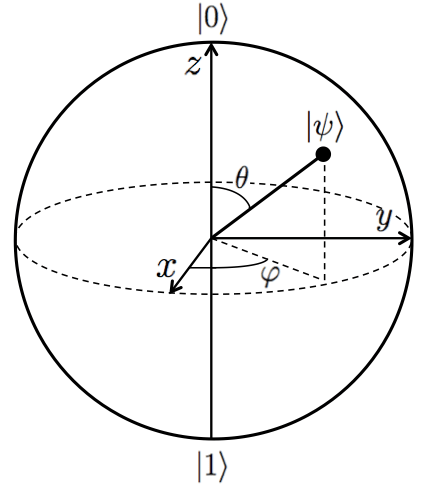
\includegraphics[scale=0.30]{img/EsferadeBloch.png}
\captionof{figure}{La esfera de Bloch representa todos los posibles estados cuánticos de un qubit.}
\label{fig:esferaBloch}
\end{center}
\noindent
Con esto en mente, podemos entender mejor cómo los qubits permiten realizar cálculos que son imposibles o ineficientes para las computadoras clásicas. Por ejemplo, mientras un bit clásico solo almacena un único valor en un momento dado, un qubit en superposición puede representar múltiples valores simultáneamente.
\section{Partículas}
\noindent 
Para empezar esta guía, quiero comenzar por la base de todo. Sería inútil hablar sobre computación cuántica y qubits sin entender realmente con qué estamos trabajando. No se preocupen, este no será un capítulo muy teórico ni estará lleno de fórmulas matemáticas (que, obviamente, son necesarias), pero trataré de explicarlo con palabras más naturales para todos. Además, este tema es sumamente amplio, por lo cual solo se explicará lo fundamental y necesario para comprender mejor los conceptos utilizados en la computación cuántica. Esto no reemplaza el aprendizaje a un nivel más profundo sobre física (recomiendo leer el libro *Atomic Theory and the Description of Nature* de Niels Bohr); es solamente una introducción a este fascinante mundo.\\

\noindent 
¡Bienvenidos al mundo cuántico, donde si no estás entendiendo nada, es porque lo estás entendiendo todo!

\noindent 
Al principio podríamos pensar que el universo se rige únicamente por las leyes que conocemos, como la ley de la gravedad descubierta por Isaac Newton. Esta idea parece lógica, ya que convivimos con la gravedad todos los días y observamos su comportamiento constantemente. Sin embargo, aunque esta ley explica muchos fenómenos cotidianos y astronómicos, no abarca por completo todos los aspectos del universo, especialmente en escalas extremadamente grandes, como las galaxias, o extremadamente pequeñas, como las partículas subatómicas. Es en estas escalas donde estaremos enfocados.\\

\noindent 
Un ejemplo claro de estas diferencias son los seres unicelulares. Para ellos, nuestro concepto de 'arriba' y 'abajo', que nos da una orientación gracias a la gravedad, carece de relevancia. En cambio, para estos organismos, la tensión superficial tiene un papel mucho más importante que la fuerza gravitatoria. La tensión superficial es una consecuencia de la atracción entre las moléculas de un líquido, que forman una especie de 'capa elástica' en su superficie. Esta atracción es causada por una fuerza conocida como la fuerza de Van der Waals. Estas interacciones ocurren cuando los átomos y las moléculas están muy cerca unos de otros, generando una atracción que puede unirlos con cierta intensidad. A nivel molecular, las fuerzas de Van der Waals son el resultado de interacciones débiles entre dipolos eléctricos temporales o permanentes en las moléculas. Aunque estas fuerzas son mucho más débiles que los enlaces químicos como los covalentes o iónicos, son fundamentales en muchos procesos biológicos y químicos, como la adhesión entre superficies o el comportamiento de las membranas celulares.\\

\noindent 
Antes de hablar y explicar más términos, vamos a repasar un poco los más básicos y adentrarnos en lo más pequeño. Para muchos, se les puede haber olvidado qué es una partícula subatómica, qué son las moléculas, un fotón, entre otros términos. Entonces, empecemos por lo esencial.\\

\noindent 
Las partículas subatómicas son los componentes más pequeños que existen y, por ende, conforman los átomos. Entre estas partículas se incluyen los electrones, protones y neutrones, entre otras (las cuales no detallaremos aquí). Los electrones tienen una carga negativa y giran alrededor del núcleo del átomo, mientras que los protones, con carga positiva, y los neutrones, sin carga, se encuentran en el núcleo. El electrón es una partícula subatómica con carga eléctrica negativa de magnitud $-e$, donde $e = 1.602 \times 10^{-19} \, \text{C}$. Es una de las partículas fundamentales según el modelo estándar de la física de partículas y no tiene estructura interna conocida, es decir, no está compuesta por partículas más pequeñas. Posee una masa de:
\[
m_e = 9.109 \times 10^{-31} \, \text{kg}.
\]
\noindent 
El electrón participa en interacciones electromagnéticas y es responsable de la mayoría de las propiedades químicas de los átomos, ya que forma los enlaces químicos y define la configuración electrónica.\\

\noindent 
Al mencionar los átomos, es importante recordar que el átomo es la unidad básica de la materia que conserva las propiedades químicas de un elemento. Está compuesto por un núcleo central y una nube de electrones cargados eléctricamente que se mueven alrededor del núcleo, lo que le da su forma casi esférica. La carga eléctrica del electrón es de signo opuesto a la del núcleo, lo que provoca que los electrones estén fuertemente atraídos hacia él y, al mismo tiempo, se repelan mutuamente. Esta interacción obedece a la fuerza electrostática o de Coulomb, además, las leyes de movimiento de los electrones y el núcleo atómico están completamente regidas por la mecánica cuántica, por ende los átomos obedecen a estas leyes.\\

\noindent 
Prácticamente toda la masa del átomo se encuentra en el núcleo, que está compuesto por protones y neutrones, ambos considerados partículas subatómicas. Los protones son partículas con carga positiva igual a $+e$ y tienen una masa de:
\[
m_p = 1.673 \times 10^{-27} \, \text{kg}.
\]
\noindent 
Por su parte, los neutrones son partículas neutras (sin carga) con una masa ligeramente mayor que la del protón:
\[
m_n = 1.675 \times 10^{-27} \, \text{kg}.
\]
\noindent 
Es importante señalar que los protones y neutrones, colectivamente, son llamados nucleones.\\

\noindent 
Cuando varios átomos se agrupan, forman moléculas. Actualmente, se conocen más de 100 tipos de átomos (elementos), cada uno con características que los diferencian de los demás. La fuerza nuclear fuerte, mediada por los gluones, mantiene unidos a los nucleones, contrarrestando la repulsión eléctrica entre los protones. El número de protones determina el elemento químico (número atómico, $Z$), mientras que el número de neutrones define los isótopos de dicho elemento.\\

\noindent 
Es fundamental aclarar la diferencia entre masa y peso, ya que suelen confundirse. En la Tierra, los objetos tienen un peso que parece equivalente a su masa, pero esto se debe a la fuerza gravitatoria que ejerce el planeta sobre ellos. El peso, en realidad, es la fuerza con la que la gravedad atrae un objeto hacia el centro de la Tierra. En cambio, la masa es una propiedad intrínseca del objeto y no cambia, sin importar dónde se encuentre. Por ejemplo, en una nave espacial lejos de la influencia gravitacional de la Tierra, la masa de un objeto sigue siendo la misma, pero su peso sería prácticamente nulo.\\

\noindent 
Los electrones orbitan alrededor del núcleo en niveles de energía cuantizados, definidos por los principios de la mecánica cuántica. Los átomos de plata tienen 47 electrones: dos en la órbita más interna, ocho en la siguiente, luego dieciocho en cada uno de los dos niveles siguientes. Esto deja un único electrón en la órbita más externa. Los átomos de oro tienen 79 electrones; a diferencia del átomo de plata, este tiene 6 niveles, en los cuales: el primer nivel cuenta con dos electrones, ocho en el segundo nivel, dieciocho en el tercero, 32 en el cuarto, dieciocho en el quinto e, igual que el átomo de plata, el último nivel o la órbita más externa cuenta con un único electrón.\\

\noindent 
También es importante saber qué es un fotón. No es más que una partícula elemental de la luz y de todas las formas de radiación electromagnética. Es un bosón sin masa que actúa como el cuanto de energía del campo electromagnético. Su energía está relacionada con la frecuencia de la radiación según:
\[
E = h v,
\]
\noindent 
donde $v$ es la frecuencia de la onda electromagnética. Además, el fotón tiene momento lineal dado por:
\[
p = \frac{h}{\lambda},
\]
\noindent 
donde $\lambda$ es la longitud de onda. Los fotones no tienen carga eléctrica y viajan a la velocidad de la luz en el vacío:
\[
c = 3.00 \times 10^8 \, \text{m/s}.
\]
\noindent 
En una vista más general, una partícula es una entidad que puede describirse mediante propiedades como masa, carga y momento. Las partículas subatómicas se dividen en fermiones y bosones. Los fermiones constituyen la materia (electrones, protones, neutrones, quarks, etc.) y obedecen el principio de exclusión de Pauli, mientras que los bosones median las interacciones fundamentales (fotones, gluones, bosones $W$ y $Z$, etc.).

\subsection*{Modelo atómico de Niels Bohr}
\noindent 
hablaremos un poco sobre el modelo atómico propuesto en 1913 por el físico danés Niels Bohr, el cual representó una importante evolución en la descripción del átomo al introducir formalmente el concepto de cuantización de energía a través de postulados fundamentales. Este modelo se basó en los principios de la mecánica cuántica y la teoría del espectro atómico, estableciendo que los electrones pueden ocupar únicamente ciertas órbitas alrededor del núcleo, denominadas niveles de energía cuantizados, en las cuales no emiten radiación electromagnética debido a su movimiento acelerado. Este enfoque resolvía problemas inherentes al modelo clásico de Rutherford, que no podía explicar la estabilidad de los átomos. Además, Bohr formuló que los átomos emiten o absorben energía en forma de fotones cuando los electrones realizan transiciones entre estos niveles de energía, lo que permite interpretar con precisión los espectros de emisión y absorción característicos de cada elemento, según la relación:

\[
E = hv
\]
\noindent 
$h$ es la constante de Planck y $v$ la frecuencia del fotón emitido o absorbido.\\[0.5em]
\noindent 
En este modelo, los electrones giran alrededor en órbitas del núcleo del átomo sin irradiar energía. Ahora bien, no toda órbita para el electrón está permitida: ellos ocupan la órbita de menor energía posible o la órbita más cercana posible al núcleo. El electrón solo emite o absorbe energía en los saltos de una órbita permitida a otra. Al realizar ese cambio, emite o absorbe un fotón cuya energía es la diferencia de energía entre ambos niveles, dada por:

\[
\Delta E = E_f - E_i = h v
\]
\noindent 
$E_f$ y $E_i$ son las energías de los niveles final e inicial, respectivamente.\\[0.5em]
\noindent 
Según Bohr, las órbitas permitidas están determinadas por la cuantización del momento angular del electrón, descrita por la fórmula:

\[
L = n \hbar = n \frac{h}{2\pi}, \quad n = 1, 2, 3, \ldots
\]
\noindent 
$L$ es el momento angular, $n$ es el número cuántico principal y $\hbar = \frac{h}{2\pi}$ es la constante de Planck reducida.\\[0.5em]
\noindent 
La energía total de un electrón en una órbita permitida está dada por:

\[
E_n = -\frac{Z^2 e^4}{8 \varepsilon_0^2 h^2 n^2}
\]
\noindent 
Este modelo permitió explicar el espectro de emisión del hidrógeno, cuya longitud de onda está dada por la fórmula de Rydberg:

\[
\frac{1}{\lambda} = R_H \left( \frac{1}{n_i^2} - \frac{1}{n_f^2} \right)
\]
\noindent
El modelo estándar de la física de partículas clasifica las partículas fundamentales en dos categorías principales:\\[0.5em]
\noindent
\textbf{Fermiones:} Constituyen la materia. Obedecen al principio de exclusión de Pauli y tienen espín semi-entero $(\frac{1}{2})$.
    \begin{itemize}
        \item \textbf{Quarks:} Se combinan para formar hadrones como protones y neutrones. Hay seis tipos: arriba ($u$), abajo ($d$), encanto ($c$), extraño ($s$), cima ($t$) y fondo ($b$).
        \item \textbf{Leptones:} Incluyen el electrón ($e^-$), el muón ($\mu^-$), el tauón ($\tau^-$), y sus correspondientes neutrinos ($\nu_e$, $\nu_\mu$, $\nu_\tau$).
    \end{itemize}
\noindent
\textbf{Bosones:} Median las interacciones fundamentales. Tienen espín entero.
    \begin{itemize}
        \item \textbf{Fotón ($\gamma$):} Mediador de la fuerza electromagnética.
        \item \textbf{Gluones ($g$):} Mediadores de la fuerza fuerte.
        \item \textbf{Bosones $W^\pm$ y $Z^0$:} Mediadores de la fuerza débil.
        \item \textbf{Bosón de Higgs ($H$):} Responsable de dar masa a las partículas a través del mecanismo de Higgs.
    \end{itemize}

\subsection*{Dualidad Onda-Partícula}
\noindent
Un concepto fundamental en la mecánica cuántica es la dualidad onda-partícula, que establece que las partículas, como los electrones, pueden exhibir comportamientos tanto de partículas como de ondas, dependiendo de cómo se las observe o mida. Esto implica que los electrones no tienen una trayectoria definida como en la física clásica, sino que su posición y momento están descritos por una función de onda, que representa un espectro de probabilidades para encontrar al electrón en distintos lugares. No significa que el electrón esté literalmente en varios lugares a la vez, sino que, antes de ser medido, su estado está representado por una superposición cuántica de todas las posiciones posibles. Este concepto es esencial para comprender fenómenos como la interferencia y la difracción de partículas, y se describe mediante principios como la longitud de onda de De Broglie y el principio de incertidumbre de Heisenberg\\[0.5em]
\noindent
\textbf{Longitud de onda de De Broglie:}
    \[
    \lambda = \frac{h}{p},
    \]
    donde $h$ es la constante de Planck y $p$ es el momento lineal de la partícula.\\[0.5em]
\noindent
\textbf{Principio de incertidumbre de Heisenberg:}
    \[
    \Delta x \Delta p \geq \frac{\hbar}{2},
    \]
    que establece límites fundamentales en la precisión con la que se pueden medir simultáneamente la posición ($x$) y el momento ($p$) de una partícula.

\subsection*{Interacciones Fundamentales}
\noindent
En el universo, las partículas subatómicas interactúan a través de cuatro fuerzas fundamentales que determinan la estructura y dinámica de la materia. Estas fuerzas son:\\[0.5em]
\noindent
\textbf{Fuerza Gravitacional:} Actúa entre masas y es responsable de fenómenos como la formación de planetas y galaxias. Aunque universal, su efecto a escala subatómica es despreciable comparado con las demás fuerzas.\\[0.5em]
\noindent
\textbf{Fuerza Electromagnética:} Responsable de la interacción entre partículas con carga eléctrica. Es mediada por fotones y describe fenómenos como la formación de enlaces químicos y las propiedades ópticas de los materiales.\\[0.5em]
\noindent
\textbf{Fuerza Nuclear Fuerte:} Une los quarks dentro de los protones y neutrones y mantiene el núcleo atómico unido, superando la repulsión electrostática entre protones. Es mediada por los gluones.\\[0.5em]
\noindent
\textbf{Fuerza Nuclear Débil:} Responsable de procesos de desintegración nuclear, como la emisión beta. Es mediada por los bosones $W^\pm$ y $Z^0$ y juega un papel clave en la física de partículas y la cosmología.

\subsection*{Espín}
\noindent
El espín es una propiedad intrínseca de las partículas cuánticas que puede entenderse como una forma de momento angular interno. A diferencia del momento angular orbital, el espín no está asociado a un movimiento en el espacio clásico, sino que es una característica fundamental de las partículas. Matemáticamente, el espín se describe mediante un operador $S$ que cumple las mismas reglas de conmutación que el momento angular orbital $L$:
\[
[S_i, S_j] = i\hbar \epsilon_{ijk} S_k,
\]
donde $\epsilon_{ijk}$ es el símbolo de Levi-Civita, y $\hbar$ es la constante reducida de Planck. Estas relaciones indican que el espín obedece las leyes de la mecánica cuántica y tiene una naturaleza discreta.

\noindent
La magnitud del espín está dada por:
\[
S^2 = s(s+1)\hbar^2,
\]
donde $s$ es el número cuántico de espín que puede tomar valores enteros o semi-enteros. Por ejemplo, para los electrones, $s = \frac{1}{2}$. Este valor implica que el espín tiene dos posibles proyecciones sobre cualquier eje escogido.

\noindent
El espín de una partícula puede proyectarse sobre un eje, comúnmente el eje $z$, y sus posibles valores están dados por:
\[
S_z = m_s \hbar,
\]
donde $m_s$ es el número cuántico magnético de espín, que para un electrón toma valores $m_s = \pm\frac{1}{2}$. Esto significa que en un campo magnético externo, el espín de una partícula puede orientarse en una de dos direcciones discretas: hacia arriba ($m_s = +\frac{1}{2}$) o hacia abajo ($m_s = -\frac{1}{2}$).

\subsection*{El Experimento de Stern-Gerlach}
\noindent
El experimento de Stern-Gerlach fue diseñado en 1922 por Otto Stern y Walther Gerlach para estudiar la cuantización espacial del momento angular de los átomos, lo que llevó al descubrimiento del espín como una propiedad intrínseca de las partículas subatómicas.
\noindent
Un haz de átomos de plata es producido calentando una fuente que contiene el metal. Estos átomos, al ser neutros, no deberían interactuar significativamente con un campo eléctrico, pero debido a sus momentos magnéticos, interactúan con un campo magnético externo. 

Los átomos de plata son enviados a través de un campo magnético no uniforme generado por un par de imanes dispuestos de manera asimétrica, donde el campo magnético tiene una fuerte dependencia espacial en la dirección $z$. El momento magnético de los átomos interactúa con este campo, y los átomos experimentan una fuerza diferencial en función de la orientación de sus momentos magnéticos.
\noindent
El momento magnético $\boldsymbol{\mu}$ está relacionado con el espín mediante:
\[
\boldsymbol{\mu} = -g_s \mu_B \frac{{S}}{\hbar},
\]
donde $g_s$ es el factor de Landé para el espín (aproximadamente $2$ para electrones), y $\mu_B$ es el magnetón de Bohr:
\[
\mu_B = \frac{e\hbar}{2m_e}.
\]
Aquí, $e$ es la carga del electrón y $m_e$ es su masa.
\noindent
La interacción de $\boldsymbol{\mu}$ con el campo magnético ${B}$ genera una fuerza:
\[
{F} = \nabla(\boldsymbol{\mu} \cdot {B}),
\]
y dado que el campo magnético no es uniforme, esto conduce a una fuerza diferencial en la dirección $z$:
\[
F_z = \pm g_s \mu_B \frac{\partial B_z}{\partial z}.
\]
\noindent
Al llegar a una pantalla detectora, los átomos no se distribuyen de manera continua, sino que forman dos bandas discretas. Esto demuestra que la proyección del momento magnético (y, por ende, del espín) solo puede tomar ciertos valores discretos. En el caso de los átomos de plata, los momentos magnéticos provienen principalmente del espín del electrón no apareado en su capa externa, lo que genera las dos bandas observadas.
\noindent
El resultado de este experimento es una evidencia directa de la cuantización del espín. La aparición de dos bandas separadas indica que el espín tiene solo dos estados posibles ($m_s = \pm\frac{1}{2}$), lo que contradice las predicciones de la física clásica, que sugeriría una distribución continua de orientaciones.
\noindent
El espín $\frac{1}{2}$ puede representarse mediante las matrices de Pauli, $\sigma_x$, $\sigma_y$ y $\sigma_z$, que son operadores en el espacio de dos dimensiones (spinor):
\[
\sigma_x = 
\begin{pmatrix}
0 & 1 \\
1 & 0
\end{pmatrix}, \quad
\sigma_y = 
\begin{pmatrix}
0 & -i \\
i & 0
\end{pmatrix}, \quad
\sigma_z = 
\begin{pmatrix}
1 & 0 \\
0 & -1
\end{pmatrix}.
\]
El operador de espín en una dirección arbitraria ${n} = (n_x, n_y, n_z)$ está dado por:
\[
{S} \cdot {n} = \frac{\hbar}{2}(n_x \sigma_x + n_y \sigma_y + n_z \sigma_z).
\]

\end{document}
